\documentclass{optica-article}

\journal{opticajournal}
\articletype{Research Article}

\usepackage{amsmath,mathtools,booktabs}
\usepackage{lineno}
\linenumbers % Comment out for arXiv or Optica Open preprint submission.
\emergencystretch=1.5em

\graphicspath{{figures/}}

\newcommand{\braket}[2]{\langle #1 | #2 \rangle}
\newcommand{\ket}[1]{\lvert #1 \rangle}
\newcommand{\bra}[1]{\langle #1 \rvert}
\newcommand{\norm}[1]{\lVert #1 \rVert}
\newcommand{\abs}[1]{\lvert #1 \rvert}
\newcommand{\dd}{\mathrm{d}}

\begin{document}

\title{Continuous Hilbert frame theory, paraxial propagation invariance, and exact Laguerre--Gaussian expansion of finite-width perfect optical vortex beams}

\author{Sebasti\'an Ayala\authormark{*}}

\address{Independent Researcher, Cauquenes, Chile\\
ORCID: \href{https://orcid.org/0009-0003-7348-3883}{0009-0003-7348-3883}}

\email{\authormark{*}ayala.phys.ds@gmail.com}

\begin{abstract*}
Physical perfect optical vortex beams (PVBs) confine orbital angular momentum (OAM) modes to a charge-independent ring radius $R$ with finite half-width $w > 0$. We formulate finite-width PVBs within continuous Hilbert frame theory on transverse paraxial wavefields. While azimuthal OAM sectors decouple orthogonally, radial overlap induces an isotropic Gaussian convolution frame operator $S_w = G_w * \cdot$ with optimal Bessel bound $B = 1$ and sharp Paley--Wiener lower bound $A = \exp(-w^2 k_{\max}^2/2)$ on bandlimited subspaces. We derive the closed-form complex-waist Fresnel evolution of physical PVBs, proving $S_w$ and its bounds are invariant under propagation, and establish the Tikhonov-regularized dual, an exact $(p+1)$-term Laguerre--Gaussian expansion ($p \ge 0$), the WKB arcsine resolution limit, and Jacobi-theta Toeplitz Gram bounds.
\end{abstract*}

\section{Introduction}
\label{sec:intro}

Paraxial optical beams carrying orbital angular momentum (OAM) have become central tools in optical manipulation, free-space and fiber communications, and high-dimensional quantum optics since Allen \emph{et al.} showed that helical phase fronts $\exp(il\phi)$ carry $l\hbar$ of OAM per photon~\cite{Allen1992,Siegman1986,Padgett2011,Erhard2018}. In the standard orthonormal Laguerre--Gaussian ($\mathrm{LG}_{p,l}$) eigenbasis of waist $w_0$, however, both azimuthal index $l \in \mathbb{Z}$ and radial node number $p \in \mathbb{Z}_{\ge 0}$~\cite{Plick2015,Karimi2014} govern the transverse footprint through $r_{\mathrm{rms}} = w_0\sqrt{2p+\abs{l}+1}$ (with $p=0$ peak ring radius $r_{\mathrm{peak}} = w_0\sqrt{\abs{l}/2}$). This mode-dependent expansion introduces asymmetric aperture clipping and unequal waveguide coupling across OAM channels.

To decouple annular geometry from topological charge, Ostrovsky \emph{et al.}~\cite{Ostrovsky2013} and Vaity and Rusch~\cite{Vaity2015} introduced the perfect optical vortex beam (PVB), typically synthesized via optical Fourier transformation of a Bessel--Gaussian (BG) wavefield~\cite{Gori1987,Reddy2016,Jabir2016Variable}. Subsequent experimental and theoretical investigations have examined how finite annular width modifies PVB ring invariance and modal purity~\cite{Pinnell2019HowPerfect,Pinnell2019Quantitative,Yan2022Customizable}, how optical Fourier lens constraints limit ideal quantum optical vortices~\cite{Banerji2016,Barral2017}, and how finite-width PVBs enable high-efficiency ring-core fiber transmission~\cite{Villalba2023}.

In the singular Dirac-delta limit $w \to 0$, ideal PVBs form a generalized orthonormal basis inside the distributional dual of a Gel'fand rigged Hilbert space~\cite{Gelfand1964,Ferreira2026}. Every physically realizable PVB, however, carries a finite half-width $w > 0$ and finite $L^2(\mathbb{R}^2)$ norm. In recent work on twisted Gaussian Schell-model equivalence~\cite{Ferreira2026} (Appendix~D), it was noted that finite-width PVBs lose radial orthogonality and induce Gaussian spatial smoothing, while evaluating the radial projection overlap solely for nodeless ($p = 0$) modes. Several foundational questions in mathematical optics therefore remained open: (1) how finite-width PVBs are classified within continuous Hilbert frame theory~\cite{Duffin1952,Daubechies1990,Ali1993,Christensen2016,Bastiaans1980,Grochenig2016} relative to orthogonal $\mathrm{LG}_{p,l}$ bases and optical coherent states~\cite{Klauder1985,Perelomov1986,Gazeau2009,Gazeau2018,MoralesRodriguez2024OL,MoralesRodriguez2024PRA}; (2) whether their frame operator and Paley--Wiener stability bounds survive free-space paraxial Fresnel propagation; (3) how noisy frame inversion behaves under Tikhonov regularization~\cite{Engl1996}; and (4) whether an exact finite closed-form expansion $c_{l,p}(R)$ exists for arbitrary radial order $p \ge 0$, together with rigorous radial resolution criteria and uniform discrete radial sampling bounds~\cite{Bownik2026}.

This paper resolves all four questions in a self-contained operator framework. Section~\ref{sec:conventions} establishes the frame-versus-state scaling convention, exact differential radial peak shift, and $2f$ Fourier generation bridge. Section~\ref{sec:frame_theory} proves azimuthal--radial decoupling, the Gaussian convolution frame operator $S_w = G_w * \cdot$, and sharp Paley--Wiener bounds on bandlimited subspaces $\mathcal{H}_{k_{\max}}$. Section~\ref{sec:fresnel} derives the exact closed-form complex-waist Fresnel evolution of physical PVBs, proving unitary invariance of $S_w$ across all axial planes and establishing the exact scaling of wavefront-compensated Gouy-plane analyzers. Section~\ref{sec:tikhonov} constructs the Tikhonov-regularized canonical dual and validates its exact Parseval bias--variance theory on noisy $\mathrm{LG}_{2,1}$ deconvolution. Section~\ref{sec:lg_gram} derives the exact $(p+1)$-term closed-form expansion $c_{l,p}(R)$, proves the generalized radial Rayleigh limit and its WKB arcsine constant, and establishes Jacobi-theta Toeplitz conditioning bounds for discrete concentric rings. Section~\ref{sec:conclusions} concludes the paper, while detailed special-function derivations appear in Appendix~\ref{app:lg_derivation}.

\section{Physical PVB Conventions, Peak Shift, and $2f$ Fourier Generation}
\label{sec:conventions}

\subsection{Frame-versus-State Scaling and Differential Peak Shift}

At the focal waist plane $z = 0$ in cylindrical coordinates $\mathbf{r} = (r,\phi)$, a physical PVB of topological charge $l \in \mathbb{Z}$, nominal ring radius $R > 0$, and annular half-width $w > 0$ has transverse envelope~\cite{Ostrovsky2013,Vaity2015}
\begin{equation}
  \Phi_{l,R}(r,\phi) = C_0 e^{il\phi} \exp\!\left(-\frac{r^2 + R^2}{w^2}\right) I_{\abs{l}}\!\left(\frac{2Rr}{w^2}\right), \qquad C_0 = \frac{1}{w^2}\sqrt{\frac{2}{\pi}},
  \label{eq:pvb_def}
\end{equation}
where $I_{\abs{l}}$ is the modified Bessel function of the first kind. Under physical length units $\ell_0$, $C_0$ and $\Phi_{l,R}$ carry dimension $[\ell_0^{-2}]$ rather than unit $L^2(\mathbb{R}^2)$ normalization. This natural resolution-of-identity scaling ensures that for any unit-normalized wavefield $\psi \in L^2(\mathbb{R}^2)$ ($[\psi] = \ell_0^{-1}$), the analysis projection $\braket{\Phi_{l,R}}{\psi} = \allowbreak \int_{\mathbb{R}^2}\Phi_{l,R}^*(\mathbf{r})\psi(\mathbf{r})\,\dd^2\mathbf{r}$ carries dimension $[\ell_0^{-1}]$, making the polar radial energy integral $\int_0^\infty R\,\dd R\,\abs{\braket{\Phi_{l,R}}{\psi}}^2$ and the frame operator $S_w$ strictly dimensionless while fixing the optimal upper frame bound to $B = 1$.

Applying Weber's second exponential integral (Gradshteyn--Ryzhik 6.633.2~\cite{Gradshteyn2014}, analytically continued via $J_\nu(iz) = i^\nu I_\nu(z)$) gives the exact squared $L^2(\mathbb{R}^2)$ norm
\begin{equation}
  \norm{\Phi_{l,R}}_{L^2}^2 = \frac{1}{w^2}\exp\!\left(-\frac{R^2}{w^2}\right) I_{\abs{l}}\!\left(\frac{R^2}{w^2}\right) < \frac{1}{w^2}.
  \label{eq:pvb_norm}
\end{equation}
Throughout this paper, $\{\Phi_{l,R}\}$ denotes the unnormalized continuous frame elements of Eq.~\eqref{eq:pvb_def}, whereas $\psi_{l,R} = \Phi_{l,R}/\norm{\Phi_{l,R}}_{L^2}$ (dimension $[\ell_0^{-1}]$) denotes unit-normalized physical beam states used for normalized single-channel overlaps and discrete channel Gram matrices. We restrict the continuous radial index to $R > 0$; at $R = 0$, $\Phi_{l,0} \equiv 0$ for $l \neq 0$, while $\Phi_{0,0}(r) = C_0 e^{-r^2/w^2}$ is a singleton of zero $R\,\dd R$ measure.

In the thin-ring regime $x = 2Rr/w^2 \gg 1$ and $\abs{l} \ll 2R/w$, Hankel's expansion $I_{\abs{l}}(x) = (2\pi x)^{-1/2} e^x [1 - (4l^2-1)/(8x) + \mathcal{O}(x^{-2})]$ reduces Eq.~\eqref{eq:pvb_def} to $\Phi_{l,R}(r,\phi) \approx \allowbreak (w\sqrt{2\pi^2 Rr})^{-1} e^{il\phi} \allowbreak \exp[-(r-R)^2/w^2]$. Near the optical axis ($r \to 0$), this thin-ring approximation diverges as $r^{-1/2}$ whereas Eq.~\eqref{eq:pvb_def} vanishes smoothly as $r^{\abs{l}}$, explaining the finite-width imperfections quantified by Pinnell \emph{et al.}~\cite{Pinnell2019HowPerfect}. Maximizing $\abs{\Phi_{l,R}(r)}^2$ yields the exact transcendental condition $r_{\mathrm{peak}}(l) = R\,I'_{\abs{l}}(x_{\mathrm{peak}})/I_{\abs{l}}(x_{\mathrm{peak}})$ with $x_{\mathrm{peak}} = 2R r_{\mathrm{peak}}(l)/w^2$. Solving perturbatively in $\delta = (w/R)^2 \ll 1$ using $I'_{\abs{l}}(x)/I_{\abs{l}}(x) = 1 - (2x)^{-1} + (4l^2-1)/(8x^2) + \mathcal{O}(x^{-3})$ and substituting $x_{\mathrm{peak}}^{-1} = (\delta/2)[1 + \delta/4 + \mathcal{O}(\delta^2)]$ self-consistently shifts the quadratic coefficient from $(4l^2-1)/8$ to $(4l^2-3)/8$, giving $r_{\mathrm{peak}}(l) - R = -w^2/(4R) + [(4l^2-3)/32](w^4/R^3) + \mathcal{O}(w^6/R^5)$. Subtracting the $l$-independent inward curvature shift at $l = 0$ isolates the topological differential peak shift
\begin{equation}
  \Delta r_{\mathrm{peak}}(l) \equiv r_{\mathrm{peak}}(l) - r_{\mathrm{peak}}(0) \approx \frac{l^2}{8}\left(\frac{w}{R}\right)^4 R.
  \label{eq:peak_shift}
\end{equation}
At $w/R = 0.10$, Eq.~\eqref{eq:peak_shift} matches the exact transcendental root within $1.2\%$ across $l = 1\text{--}6$ ($\Delta r_{\mathrm{peak}}/R = 2.000\times 10^{-4}$ vs.\ exact $2.024\times 10^{-4}$ at $l = 4$), as illustrated in Fig.~\ref{fig:pvb_overlap}(a).

\begin{figure}[htbp]
  \centering
  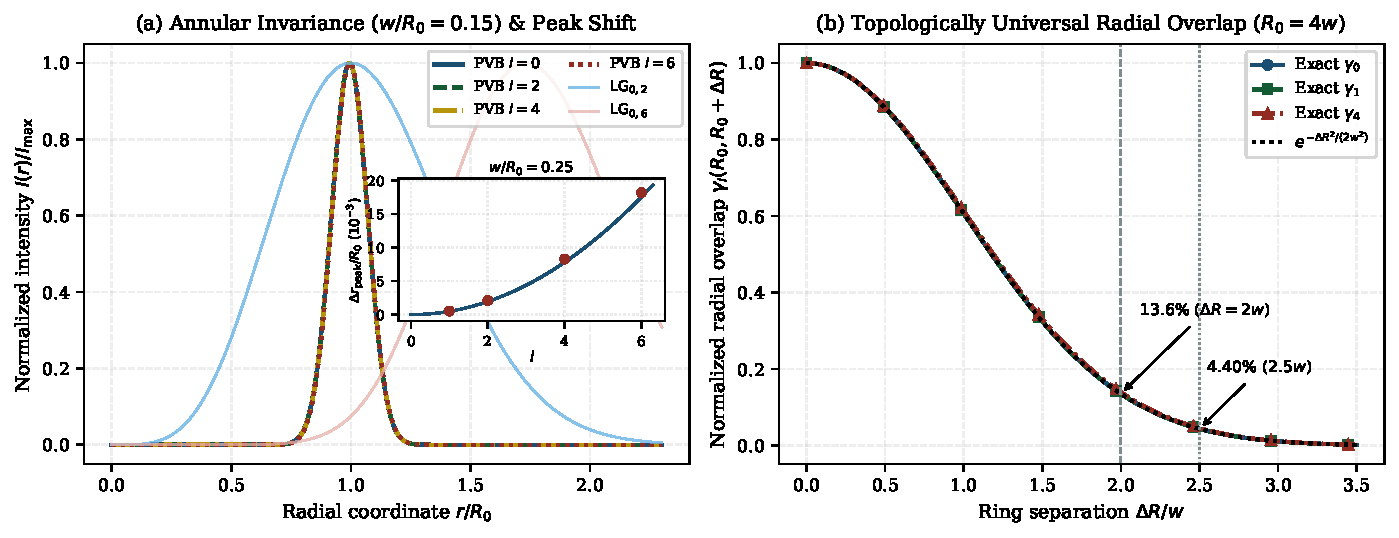
\includegraphics[width=0.98\textwidth]{fig1_pvb_overlap_shift.pdf}
  \caption{Physical PVB annular invariance and mutual radial overlap. (a) Peak-normalized radial intensity $I(r)/I_{\max}$ for physical PVBs ($w/R_0 = 0.15$) across $l = 0,2,4,6$ compared with $\mathrm{LG}_{0,l}$ ($w_0 = R_0$); inset compares the exact transcendental differential shift $\Delta r_{\mathrm{peak}}(l)/R_0$ ($w/R_0 = 0.25$, circles) against Eq.~\eqref{eq:peak_shift} (solid curve). (b) Unit-normalized radial overlap $\gamma_l(R_0, R_0+\Delta R)$ [Eq.~\eqref{eq:gamma_norm}] at $R_0 = 4w$ for $l = 0,1,4$ against the $l$-independent Gaussian asymptote $e^{-\Delta R^2/(2w^2)}$, marking $13.6\%$ at $\Delta R = 2.0\,w$ and $4.40\%$ at $\Delta R = 2.5\,w$.}
  \label{fig:pvb_overlap}
\end{figure}

\subsection{Optical $2f$ Fourier Generation and Two-Zone Propagation}

In a $2f$ optical Fourier relay using a spherical lens of focal length $f$~\cite{Vaity2015,Goodman2017}, placing an input Bessel--Gaussian beam $E_{\mathrm{BG}}(\rho,\theta) = E_0 J_l(k_r\rho)\exp(-\rho^2/w_g^2) e^{il\theta}$~\cite{Gori1987} at the front focal plane ($d_{\mathrm{in}} = f$) cancels the quadratic Fresnel phase and maps $E_{\mathrm{BG}}$ via Weber's integral directly to Eq.~\eqref{eq:pvb_def} at the back focal plane $z = 0$ (up to global phase $(-i)^{l+1} e^{2ik_0 f}$) with
\begin{equation}
  R = \frac{k_r f}{k_0}, \qquad w = \frac{2f}{k_0 w_g}, \qquad E_0 = \frac{1}{w w_g}\sqrt{\frac{2}{\pi}} = \frac{k_0}{f\sqrt{2\pi}},
  \label{eq:2f_bridge}
\end{equation}
where $k_0 = 2\pi/\lambda$ and $k_r = k_0(n_{\mathrm{ax}}-1)\beta$ is the conical radial wavevector. The relay separates two disjoint axial regimes: preceding the lens, conical BG rays clear an on-axis obstruction of radius $a_{\mathrm{obs}} \le R$ at $z_{\mathrm{heal}} \approx k_0 a_{\mathrm{obs}}/k_r \le f$ within the axicon zone $z_{\max} \approx k_0 w_g/k_r$; past the focal waist ($z > 0$), the flat-phase ring diffracts over the annular Rayleigh range $z_R^{\mathrm{ring}} = k_0 w^2/2$~\cite{Reddy2016}.

\section{Continuous Hilbert Frame Operator and Sharp Paley--Wiener Bounds}
\label{sec:frame_theory}

\subsection{Azimuthal--Radial Decoupling and Universal Radial Overlap}

Because $\{e^{il\phi}/\sqrt{2\pi}\}_{l\in\mathbb{Z}}$ forms an orthonormal basis of $L^2(S^1)$, the transverse Hilbert space decomposes orthogonally into fixed-OAM radial sectors, $L^2(\mathbb{R}^2) = \bigoplus_{l\in\mathbb{Z}} \mathcal{H}_l$. Integrating Eq.~\eqref{eq:pvb_def} via Weber's second exponential integral~\cite{Gradshteyn2014} gives the exact mutual inner product
\begin{equation}
  \braket{\Phi_{l,R}}{\Phi_{l',R'}} = \delta_{l,l'}\,\frac{1}{w^2}\exp\!\left(-\frac{R^2 + R'^2}{2w^2}\right) I_{\abs{l}}\!\left(\frac{RR'}{w^2}\right).
  \label{eq:inner_prod}
\end{equation}
Normalizing by Eq.~\eqref{eq:pvb_norm} yields the strictly positive unit-normalized radial overlap
\begin{equation}
  \gamma_l(R,R') = \braket{\psi_{l,R}}{\psi_{l,R'}} = \frac{I_{\abs{l}}(RR'/w^2)}{\sqrt{I_{\abs{l}}(R^2/w^2)\,I_{\abs{l}}(R'^2/w^2)}} \in (0,1) \qquad (R \neq R').
  \label{eq:gamma_norm}
\end{equation}
For $RR' \gg w^2$, Hankel expansion of Eq.~\eqref{eq:gamma_norm} yields $\gamma_l(R,R') \approx \exp[-(R-R')^2/(2w^2)]\{1 + [(4l^2-1)w^2(R-R')^2]/(16 R^2 R'^2)\}$, proving that radial overlap is topologically universal ($l$-independent) at leading order [Fig.~\ref{fig:pvb_overlap}(b)].

\subsection{Continuous Bessel Bound and Gaussian Convolution Kernel}

A measurable family $\{\Phi_\omega\}_{\omega\in\Omega}$ in a Hilbert space $\mathcal{H}$ with measure $\mu$ is a continuous Hilbert frame~\cite{Duffin1952,Daubechies1990,Ali1993,Christensen2016} if there exist constants $0 < A \le B < \infty$ such that $A\norm{\psi}_{\mathcal{H}}^2 \le \int_\Omega \abs{\braket{\Phi_\omega}{\psi}}^2\,\dd\mu(\omega) \le B\norm{\psi}_{\mathcal{H}}^2$ for all $\psi \in \mathcal{H}$ (and a continuous Bessel system if only $B < \infty$ holds). Adopting the index space $\Omega = \mathbb{Z}\times(0,\infty)$ with polar measure $\dd\mu(l,R) = R\,\dd R$, analysis operator $(T\psi)(l,R) = \braket{\Phi_{l,R}}{\psi}$, and non-unitary 2D Fourier convention $\widetilde{\psi}(\mathbf{k}) = \int_{\mathbb{R}^2}\psi(\mathbf{r})e^{-i\mathbf{k}\cdot\mathbf{r}}\,\dd^2\mathbf{r}$ [Plancherel identity $\braket{\phi}{\psi}_{L^2} = (2\pi)^{-2}\braket{\widetilde{\phi}}{\widetilde{\psi}}_{L^2}$], Jacobi--Anger azimuthal integration and Weber 6.633.4 give the exact 2D Fourier transform of Eq.~\eqref{eq:pvb_def}:
\begin{equation}
  \widetilde{\Phi}_{l,R}(\mathbf{k}) = \sqrt{2\pi}\,(-i)^{\abs{l}} e^{il\phi_k} \exp\!\left(-\frac{w^2 k_\perp^2}{4}\right) J_{\abs{l}}(R k_\perp),
  \label{eq:pvb_ft}
\end{equation}
where $k_\perp = \abs{\mathbf{k}}$. Expanding $\widetilde{\psi}(k_\perp,\phi_k) = \sum_{l\in\mathbb{Z}}\widetilde{\psi}_l(k_\perp)e^{il\phi_k}$, Plancherel's theorem expresses $(T\psi)(l,R) = (2\pi)^{-1/2} i^{\abs{l}}\,\mathrm{H}_{\abs{l}}[e^{-w^2 k_\perp^2/4}\widetilde{\psi}_l](R)$ directly in terms of the unitary order-$\abs{l}$ Hankel transform $\mathrm{H}_{\abs{l}}$. Integrating $\abs{(T\psi)(l,R)}^2 R\,\dd R$ and summing over $l \in \mathbb{Z}$ immediately yields
\begin{equation}
  \norm{T\psi}_{L^2(\Omega,\mu)}^2 = \int_{\mathbb{R}^2} e^{-w^2 k_\perp^2/2}\abs{\widetilde{\psi}(\mathbf{k})}^2\,\frac{\dd^2\mathbf{k}}{(2\pi)^2} \le \norm{\psi}_{L^2}^2,
  \label{eq:bessel_identity}
\end{equation}
establishing that $\{\Phi_{l,R}\}$ is a continuous Bessel system on $L^2(\mathbb{R}^2)$ with optimal upper bound $B = 1$ (saturated by wavepackets concentrated near $k_\perp = 0$).

By polarization of Eq.~\eqref{eq:bessel_identity}, the continuous frame operator $S_w = T^* T$, defined weakly by $S_w\psi = \sum_{l\in\mathbb{Z}}\int_0^\infty R\,\dd R\,\braket{\Phi_{l,R}}{\psi}\Phi_{l,R}$, acts on $L^2(\mathbb{R}^2)$ as the isotropic Gaussian convolution
\begin{equation}
  (S_w\psi)(\mathbf{r}) = (G_w * \psi)(\mathbf{r}), \qquad G_w(\mathbf{r}) = \frac{1}{2\pi w^2}\exp\!\left(-\frac{\abs{\mathbf{r}}^2}{2w^2}\right), \qquad \widetilde{G}_w(k_\perp) = e^{-w^2 k_\perp^2/2}.
  \label{eq:frame_conv}
\end{equation}
Hence $S_w$ is positive, bounded ($\norm{S_w} = 1$), and self-adjoint with purely continuous spectrum $\sigma(S_w) = [0,1]$ accumulating at $0$ as $k_\perp \to \infty$ (non-compact on unconstrained $\mathbb{R}^2$, though Hilbert--Schmidt when spatially windowed to a finite pupil). This places the Gaussian smoothing action noted in Appendix~D of Ref.~\cite{Ferreira2026} into exact global operator form.

\subsection{Sharp Paley--Wiener Frame Bounds on Bandlimited Optical Subspaces}

On unconstrained $L^2(\mathbb{R}^2)$, $A = \inf_{k_\perp \ge 0}\widetilde{G}_w(k_\perp) = 0$, so $S_w^{-1}$ is unbounded and $S_w^{-1}\Phi_{l,R} \notin L^2(\mathbb{R}^2)$ because $e^{+w^2 k_\perp^2/2}\widetilde{\Phi}_{l,R}(\mathbf{k}) \propto e^{+w^2 k_\perp^2/4}J_{\abs{l}}(R k_\perp)$ diverges exponentially. Every physical optical instrument, however, imposes a finite numerical aperture $\mathrm{NA}$, restricting fields to the Paley--Wiener reproducing-kernel Hilbert space~\cite{PaulsenRaghupathi2016} $\mathcal{H}_{k_{\max}} = \{\psi \in L^2(\mathbb{R}^2) : \operatorname{supp}(\widetilde{\psi}) \subseteq \{k_\perp \le k_{\max}\}\}$ with cutoff $k_{\max} = k_0\mathrm{NA}$ and orthogonal Fourier-cutoff projector $P_{k_{\max}}$.

For all $\psi \in \mathcal{H}_{k_{\max}}$, $P_{k_{\max}}\psi = \psi$ gives $\braket{P_{k_{\max}}\Phi_{l,R}}{\psi} = \braket{\Phi_{l,R}}{\psi}$, so the projected family $\{P_{k_{\max}}\Phi_{l,R}\}$ forms a bona fide continuous Hilbert frame on $\mathcal{H}_{k_{\max}}$ with restricted frame operator $S_{w,k_{\max}} = P_{k_{\max}} S_w P_{k_{\max}}\big|_{\mathcal{H}_{k_{\max}}}$ and frame bounds
\begin{equation}
  A(w,k_{\max}) = \exp\!\left(-\frac{w^2 k_{\max}^2}{2}\right) > 0, \qquad B = 1, \qquad \kappa(S_{w,k_{\max}}) = \frac{B}{A} = \exp\!\left(\frac{w^2 k_{\max}^2}{2}\right).
  \label{eq:pw_bounds}
\end{equation}
Sharpness of both bounds is verified analytically by unit-norm Fourier-annulus test states $\widetilde{\psi}_\epsilon^{(+)}(\mathbf{k}) = 2\pi(\pi\epsilon^2)^{-1/2}\allowbreak\mathbf{1}_{\{0<k_\perp\le\epsilon\}}$ and $\widetilde{\psi}_\epsilon^{(-)}(\mathbf{k}) = 2\pi[\pi\epsilon(2k_{\max}-\epsilon)]^{-1/2}\allowbreak\mathbf{1}_{\{k_{\max}-\epsilon\le k_\perp\le k_{\max}\}}$, whose exact Rayleigh quotients yield $2(1-e^{-w^2\epsilon^2/2})/(w^2\epsilon^2) \to 1$ and $2[e^{-w^2(k_{\max}-\epsilon)^2/2} - e^{-w^2 k_{\max}^2/2}]/[w^2\epsilon(2k_{\max}-\epsilon)] \to e^{-w^2 k_{\max}^2/2}$ as $\epsilon \to 0^+$. On $\mathcal{H}_{k_{\max}}$, the canonical dual frame elements $\widetilde{\Phi}_{l,R} = S_{w,k_{\max}}^{-1}P_{k_{\max}}\Phi_{l,R} \in \mathcal{H}_{k_{\max}}$ are rigorously bounded.

Table~\ref{tab:frame_hierarchy} contrasts Dirac PVBs, physical PVBs, orthogonal $\mathrm{LG}_{p,l}$ modes, and optical coherent states~\cite{Klauder1985,Perelomov1986,Gazeau2009,Gazeau2018,MoralesRodriguez2024OL,MoralesRodriguez2024PRA}. Fundamental wave optics forbids taking $w \to 0$: transverse wavevector variance diverges as $\langle k_\perp^2\rangle \sim w^{-2}$, beam quality degrades as $M^2 \sim R/w$, and any finite pupil diameter $D$ enforces the diffraction bound $w \ge 2\lambda f/(\pi D)$~\cite{Barral2017}.

\begin{table}[htbp]
  \centering
  \caption{Structural Comparison of Ideal Dirac PVBs, Physical Finite-Width PVBs, $\mathrm{LG}_{p,l}$ Eigenmodes, and Coherent States}
  \label{tab:frame_hierarchy}
  \scriptsize
  \renewcommand{\arraystretch}{1.16}
  \begin{tabularx}{\textwidth}{@{}lXXXX@{}}
  \toprule
  \textbf{Property} & \textbf{Dirac PVB ($w=0$)} & \textbf{Physical PVB ($w>0$)} & \textbf{$\mathrm{LG}_{p,l}$ Modes} & \textbf{Coherent States $\ket{\alpha}$} \\
  \midrule
  Function space & Rigged dual $\Phi^\times$ ($\notin L^2$) & $L^2(\mathbb{R}^2)$ (frame on $\mathcal{H}_{k_{\max}}$) & $L^2(\mathbb{R}^2)$ (complete ONB) & Bargmann--Fock $L^2$ \\
  Orthogonality & $\delta_{l,l'}\delta(R-R')/R$ & $\delta_{l,l'}$ in $l$; $\gamma_l(R,R')\in(0,1)$ & $\delta_{p,p'}\delta_{l,l'}$ & $\abs{\braket{\alpha}{\beta}} = e^{-\abs{\alpha-\beta}^2/2}$ \\
  Frame bounds & Generalized ONB & $A=e^{-w^2 k_{\max}^2/2},\; B=1$ & Tight ($A=B=1$) & Tight ($A=B=1$, $\dd^2\alpha/\pi$) \\
  Dual / inversion & Self-dual ($\notin L^2$) & $S_w = G_w * \cdot$; Paley--Wiener / Tikhonov & Self-dual ($S=\mathbb{I}$) & Self-dual ($S=\mathbb{I}$) \\
  Radial footprint & Singular ($\langle k_\perp^2\rangle=\infty$) & $l$-invariant $R$ [$\Delta r_{\mathrm{peak}}\propto (w/R)^4 R$] & $w_0\sqrt{2p+\abs{l}+1}$ & Displaced phase-space packet \\
  \bottomrule
  \end{tabularx}
\end{table}

\section{Exact Paraxial Fresnel Propagation Invariance}
\label{sec:fresnel}

Under free-space paraxial evolution $(2ik_0\partial_z + \nabla_\perp^2)\psi = 0$ (omitting the global carrier $e^{ik_0 z}$), the unitary Fresnel propagator $\mathcal{U}_z$ acts in spatial-frequency space as multiplication by $\exp(-iz k_\perp^2/(2k_0))$~\cite{Goodman2017}. Multiplying Eq.~\eqref{eq:pvb_ft} by $\exp(-iz k_\perp^2/(2k_0))$ shifts $w^2/4$ to the complex annular waist parameter
\begin{equation}
  w_c^2(z) \equiv w^2\!\left(1 + i\frac{z}{z_R^{\mathrm{ring}}}\right), \qquad z_R^{\mathrm{ring}} = \frac{k_0 w^2}{2}.
  \label{eq:wc_z}
\end{equation}
Because $\operatorname{Re}[w_c^2(z)/4] = w^2/4 > 0$ strictly for all $z \in \mathbb{R}$, inverting the order-$\abs{l}$ Hankel transform via Weber's second exponential integral~\cite{Gradshteyn2014} yields the exact closed-form propagated physical PVB at every axial plane $z$:
\begin{equation}
  \Phi_{l,R}^{(z)}(r,\phi) \equiv (\mathcal{U}_z\Phi_{l,R})(r,\phi) = \frac{1}{w_c^2(z)}\sqrt{\frac{2}{\pi}}\,e^{il\phi}\exp\!\left(-\frac{r^2 + R^2}{w_c^2(z)}\right) I_{\abs{l}}\!\left(\frac{2Rr}{w_c^2(z)}\right).
  \label{eq:pvb_fresnel}
\end{equation}
Separating $1/w_c^2(z) = w^{-2}(z) - i k_0/[2R_c^{\mathrm{ring}}(z)]$ reveals smooth diffraction broadening $w(z) = w\sqrt{1 + (z/z_R^{\mathrm{ring}})^2}$ accompanied by annular wavefront curvature $R_c^{\mathrm{ring}}(z) = z[1 + (z_R^{\mathrm{ring}}/z)^2]$. Across $l \in \{0,1,3\}$ and $z/z_R^{\mathrm{ring}} \in \{0, 0.5, 1.0, 2.5\}$, Eq.~\eqref{eq:pvb_fresnel} matches direct 40-digit inverse Hankel quadrature to $5.27\times 10^{-23}$ relative error and $512\times 512$ 2D-FFT angular-spectrum propagation to $4.73\times 10^{-16}$ relative $L^2$ error [Fig.~\ref{fig:fresnel_bounds}(a)].

Because $S_w$, $\mathcal{U}_z$, and $P_{k_{\max}}$ are simultaneously diagonal radial Fourier multipliers, they commute pairwise identically:
\begin{equation}
  [S_w, \mathcal{U}_z] = 0, \qquad [P_{k_{\max}}, \mathcal{U}_z] = 0 \implies S_w^{(z)} \equiv \mathcal{U}_z S_w \mathcal{U}_z^\dagger = S_w.
  \label{eq:fresnel_commute}
\end{equation}
Two physical consequences follow immediately. First, the propagated PVB family $\{\Phi_{l,R}^{(z)}\}$ at \emph{any} axial plane $z$ generates the identical frame operator $S_w$ and retains the exact sharp Paley--Wiener frame bounds $A(w,k_{\max}) = \exp(-w^2 k_{\max}^2/2)$ and $B = 1$, while unitary invariance preserves every co-propagated modal overlap $\braket{\Phi_{l,R}^{(z)}}{\psi_{p,l}(z)} = \braket{\Phi_{l,R}}{\psi_{p,l}(0)} = c_{l,p}(R)$ (verified by 2D FFT to $6.27\times 10^{-16}$).

Second, if an $\mathrm{LG}_{p,l}$ beam of Rayleigh range $z_R = k_0 w_0^2/2$ propagates to plane $z_m$ (expanding by $\sigma_m = \sqrt{1+(z_m/z_R)^2}$ with wavefront radius $R_c(z_m) = z_m[1+(z_R/z_m)^2]$ and Gouy phase $\vartheta_m = \arctan(z_m/z_R)$) and is projected instead onto a \emph{waist-rescaled, lens-compensated} PVB analyzer, dimensional scaling of Eq.~\eqref{eq:pvb_def} obeys $\Phi_{l,\sigma_m R}(r,\phi;\,\sigma_m w) = \sigma_m^{-2}\Phi_{l,R}(r/\sigma_m,\phi;\,w)$. Defining the compensated analyzer with prefactor $\sigma_m^{+1}$,
\begin{equation}
  \phi_{l,R}^{(m)}(r,\phi) \equiv \sigma_m\,\exp\!\left(+\frac{i k_0 r^2}{2 R_c(z_m)}\right)\Phi_{l,\sigma_m R}(r,\phi;\,\sigma_m w),
  \label{eq:gouy_analyzer}
\end{equation}
cancels the Jacobian factor $\sigma_m^2$ under $\mathbf{r} = \sigma_m\mathbf{r}'$ and yields the exact Gouy-phase-modulated frame coefficient
\begin{equation}
  \braket{\phi_{l,R}^{(m)}}{\psi_{p,l}(z_m)} = e^{-i(2p+\abs{l}+1)\vartheta_m}\,c_{l,p}(R),
  \label{eq:gouy_projection}
\end{equation}
verified independently via 2D FFT to $5.78\times 10^{-16}$ relative error. Equation~\eqref{eq:gouy_projection} provides the exact operator bridge between static waist-plane expansions and multi-plane Gouy-phase radial state diagnostics.

\begin{figure}[htbp]
  \centering
  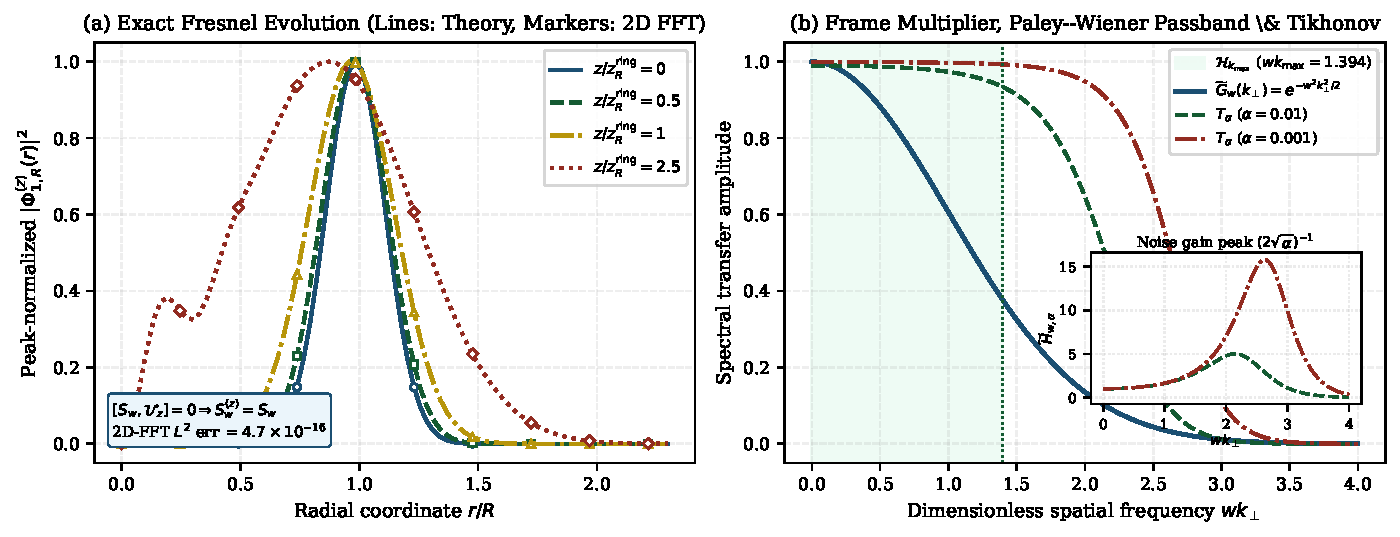
\includegraphics[width=0.98\textwidth]{fig2_fresnel_frame_bounds.pdf}
  \caption{Fresnel propagation invariance and spectral frame bounds. (a) Peak-normalized intensity $|\Phi_{1,R}^{(z)}(r)|^2$ ($w/R = 0.25$) across $z/z_R^{\mathrm{ring}} \in \{0, 0.5, 1.0, 2.5\}$: closed-form Eq.~\eqref{eq:pvb_fresnel} (curves) matches $512\times 512$ 2D-FFT propagation (markers) to $4.7\times 10^{-16}$ while $S_w^{(z)} = S_w$ stays invariant. (b) Frame Fourier multiplier $\widetilde{G}_w(k_\perp)$, Tikhonov transfer $T_{\alpha_{\mathrm{reg}}}(k_\perp)$ ($\alpha_{\mathrm{reg}} = 10^{-2}, 10^{-3}$), and Paley--Wiener passband $w k_{\max} = 1.394$ ($A = 0.378, \kappa = 2.64$); inset shows the noise-gain peak $\widetilde{H}_{\max} = (2\sqrt{\alpha_{\mathrm{reg}}})^{-1}$.}
  \label{fig:fresnel_bounds}
\end{figure}

\section{Tikhonov-Regularized Canonical Dual and Noisy $\mathrm{LG}_{2,1}$ Deconvolution}
\label{sec:tikhonov}

When reconstructing a wavefield from noisy frame measurements $\psi_{\mathrm{meas}} = S_w\psi + \varepsilon$, direct Paley--Wiener inversion multiplies high-frequency noise by $\exp(+w^2 k_\perp^2/2)$, causing severe amplification whenever $w k_{\max} \gtrsim 1$. Minimizing the Tikhonov functional $\norm{S_w\psi - \psi_{\mathrm{meas}}}_{L^2}^2 + \alpha_{\mathrm{reg}}\norm{\psi}_{L^2}^2$ ($\alpha_{\mathrm{reg}} > 0$)~\cite{Engl1996} via its Hilbert-space Fr\'echet derivative yields the bounded regularized canonical dual operator
\begin{equation}
  S_{w,\alpha_{\mathrm{reg}}}^{-1} = \left(S_w^2 + \alpha_{\mathrm{reg}}\mathbb{I}\right)^{-1} S_w, \qquad \norm{S_{w,\alpha_{\mathrm{reg}}}^{-1}} \le \frac{1}{2\sqrt{\alpha_{\mathrm{reg}}}}.
  \label{eq:tikhonov_op}
\end{equation}
Because $[S_w, P_{k_{\max}}] = 0$, Eq.~\eqref{eq:tikhonov_op} leaves $\mathcal{H}_{k_{\max}}$ invariant and acts in Fourier space via $\mathcal{F}\{S_{w,\alpha_{\mathrm{reg}}}^{-1}\psi_{\mathrm{meas}}\}(\mathbf{k}) = T_{\alpha_{\mathrm{reg}}}(k_\perp)\widetilde{\psi}(\mathbf{k}) + \widetilde{H}_{w,\alpha_{\mathrm{reg}}}(k_\perp)\widetilde{\varepsilon}(\mathbf{k})$, with signal shrinkage $T_{\alpha_{\mathrm{reg}}}(k_\perp) = \widetilde{G}_w^2/(\widetilde{G}_w^2 + \alpha_{\mathrm{reg}})$ and noise multiplier
\begin{equation}
  \widetilde{H}_{w,\alpha_{\mathrm{reg}}}(k_\perp) = \frac{e^{-w^2 k_\perp^2/2}}{e^{-w^2 k_\perp^2} + \alpha_{\mathrm{reg}}}.
  \label{eq:noise_mult}
\end{equation}
Writing $\widetilde{H}_{w,\alpha_{\mathrm{reg}}} = (g + \alpha_{\mathrm{reg}}/g)^{-1}$ with $g = \widetilde{G}_w(k_\perp)$, the arithmetic--geometric mean inequality proves that for $\alpha_{\mathrm{reg}} \in (0,1)$, $\widetilde{H}_{w,\alpha_{\mathrm{reg}}}$ attains its global peak $\widetilde{H}_{\max} = (2\sqrt{\alpha_{\mathrm{reg}}})^{-1}$ at $k_{\mathrm{peak}} = w^{-1}\sqrt{\ln(1/\alpha_{\mathrm{reg}})}$ [Fig.~\ref{fig:fresnel_bounds}(b) inset], rolling off exponentially only for $k_\perp \gg k_{\mathrm{peak}}$.

To benchmark this regularized inversion quantitatively, consider recovering the two-node mode $\mathrm{LG}_{2,1}$ ($\norm{\psi_{2,1}}_{L^2} = 1$, $w/w_0 = 0.25$, $w k_{\max} = 3.0$) from bandlimited additive white Gaussian noise $\varepsilon \in \mathcal{H}_{k_{\max}}$ of passband power $P_\varepsilon = 0.01$ ($\mathrm{SNR} = 20\,\mathrm{dB}$, spectral density $\sigma_\varepsilon^2 = 4\pi P_\varepsilon/k_{\max}^2$). With $u = w_0^2 k_\perp^2/2$, $a = w^2/w_0^2$, and normalized spectral density $\rho_{p,l}(u) = [p!/(p+\abs{l})!]u^{\abs{l}}e^{-u}[L_p^{\abs{l}}(u)]^2$, Parseval's identity splits the mean-square error $\mathrm{MSE}(\alpha_{\mathrm{reg}}) = \mathbb{E}[\norm{\hat{\psi}_{\alpha_{\mathrm{reg}}} - \psi_{2,1}}_{L^2}^2] = \mathrm{Bias}^2 + \mathrm{Var}$ in closed form:
\begin{align}
  \mathrm{Bias}^2(\alpha_{\mathrm{reg}}) &= \int_0^\infty \left[\frac{\alpha_{\mathrm{reg}}}{e^{-2au}+\alpha_{\mathrm{reg}}}\right]^2 \rho_{2,1}(u)\,\dd u, \nonumber \\
  \mathrm{Var}(\alpha_{\mathrm{reg}}) &= \frac{P_\varepsilon}{(w k_{\max})^2}\left[\frac{1}{e^{-w^2 k_{\max}^2}+\alpha_{\mathrm{reg}}} - \frac{1}{1+\alpha_{\mathrm{reg}}}\right],
  \label{eq:parseval_mse}
\end{align}
where the variance integral closes exactly via the substitution $y = e^{-w^2 k_\perp^2}$. Unregularized Paley--Wiener inversion ($\alpha_{\mathrm{reg}} = 0$) amplifies passband-edge noise by $e^9 \approx 8103$, giving $\mathrm{MSE}(0) = P_\varepsilon(e^9 - 1)/9 = 9.0023$. Minimizing Eq.~\eqref{eq:parseval_mse} gives the unique optimum $\alpha_{\mathrm{reg}}^{\mathrm{opt}} = 0.04902$, reducing total error to $\mathrm{MSE}_{\min} = 0.03481$ ($\mathrm{Bias}^2 = 0.01326$, $\mathrm{Var} = 0.02155$) --- a $258.6\times$ ($24.13\,\mathrm{dB}$) suppression that agrees with 40-trial $256\times 256$ 2D-FFT Monte Carlo simulations ($0.03488 \pm 0.00013$) and cleanly restores both radial phase-flip nodes (Fig.~\ref{fig:tikhonov_lg21}).

\begin{figure}[htbp]
  \centering
  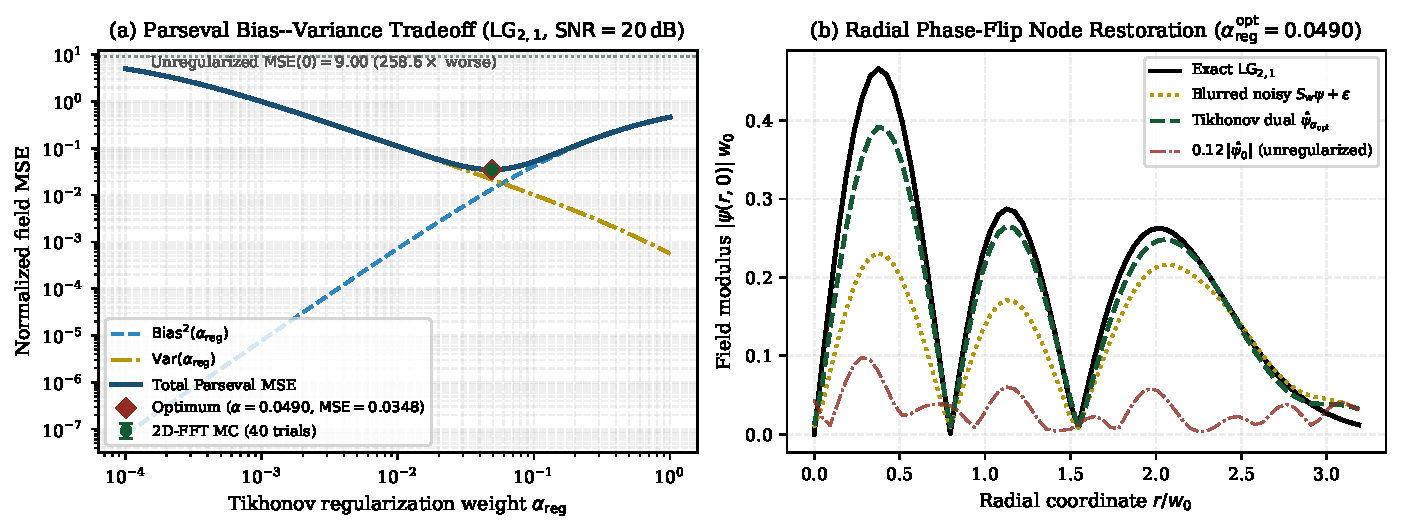
\includegraphics[width=0.98\textwidth]{fig3_tikhonov_lg21_deconv.pdf}
  \caption{Tikhonov-regularized PVB dual reconstruction of noisy $\mathrm{LG}_{2,1}$ ($w/w_0 = 0.25$, $w k_{\max} = 3.0$, $P_\varepsilon = 0.01$, $\mathrm{SNR} = 20\,\mathrm{dB}$). (a) Exact Parseval $\mathrm{Bias}^2$, variance, and total MSE [Eq.~\eqref{eq:parseval_mse}] versus $\alpha_{\mathrm{reg}}$ with 40-trial 2D-FFT Monte Carlo validation at $\alpha_{\mathrm{reg}}^{\mathrm{opt}} = 0.04902$, achieving $258.6\times$ ($24.13\,\mathrm{dB}$) MSE suppression. (b) Single-realization radial slice comparing exact $\mathrm{LG}_{2,1}$, noisy blurred input, optimal Tikhonov recovery restoring both radial nodes, and rescaled unregularized blow-up.}
  \label{fig:tikhonov_lg21}
\end{figure}

\section{Exact $\mathrm{LG}_{p,l}$ Expansion, Radial Resolution Limit, and Discrete Gram Spectrum}
\label{sec:lg_gram}

\subsection{Exact $(p+1)$-Term Closed-Form Expansion of $\mathrm{LG}_{p,l}$ Modes ($p \ge 0$)}

For an arbitrary unit-normalized Laguerre--Gaussian mode $\psi_{p,l}(r,\phi) = N_{p,l}(\sqrt{2}r/w_0)^{\abs{l}}\allowbreak L_p^{\abs{l}}(2r^2/w_0^2)\allowbreak e^{-r^2/w_0^2 + il\phi}$ with $N_{p,l} = \sqrt{2p!/[\pi(p+\abs{l})!]}/w_0$~\cite{Allen1992,Plick2015,Karimi2014}, expanding $L_p^{\abs{l}}$ into powers of $r^{2m}$, integrating term by term via Gradshteyn--Ryzhik formula 6.631.1~\cite{Gradshteyn2014}, and applying Kummer's confluent hypergeometric transformation (Appendix~\ref{app:lg_derivation}) yields the exact $(p+1)$-term closed-form PVB frame projection for all $p \ge 0$ and $l \in \mathbb{Z}$:
\begin{equation}
  c_{l,p}(R) = \braket{\Phi_{l,R}}{\psi_{p,l}} = \mathcal{A}_{p,l}(R)\sum_{m=0}^{p} (-1)^m \binom{p+\abs{l}}{p-m} \xi^m L_m^{\abs{l}}(-\zeta_R),
  \label{eq:c_lp_exact}
\end{equation}
where $\xi = 2w^2/(w_0^2+w^2)$, $\zeta_R = R^2 w_0^2/[w^2(w_0^2+w^2)]$, and
\begin{equation}
  \mathcal{A}_{p,l}(R) = 2^{\abs{l}/2+1}\sqrt{\frac{p!}{(p+\abs{l})!}}\,\frac{R^{\abs{l}} w_0^{\abs{l}+1}}{(w_0^2+w^2)^{\abs{l}+1}}\exp\!\left(-\frac{R^2}{w_0^2+w^2}\right).
  \label{eq:A_pref}
\end{equation}
These coefficients synthesize the frame-smoothed field identically via $(S_w\psi_{p,l})(\mathbf{r}) = \allowbreak \int_0^\infty R\,\dd R\,c_{l,p}(R)\Phi_{l,R}(\mathbf{r})$, generalizing the $p = 0$ formula of Ref.~\cite{Ferreira2026} (Appendix~D) to arbitrary radial orders and reducing oscillatory 2D overlap integrals to an $\mathcal{O}(p)$ three-term recurrence. Across a 36-point benchmark ($l \in \{0,1,4\}$, $p = 0\text{--}3$, $R/w_0 \in \{0.5, 1.0, 1.8\}$, $w/w_0 = 0.25$), Eq.~\eqref{eq:c_lp_exact} matches direct adaptive quadrature to maximum absolute error $1.08\times 10^{-15}$ and relative error $2.48\times 10^{-14}$ [Fig.~\ref{fig:lg_gram}(a)].

\subsection{Radial Nodal Washout and Universal WKB Arcsine Resolution Limit}

Gaussian smoothing by $S_w$ attenuates the $p$ concentric radial phase-flip nodes of $\psi_{p,l}$ once $w$ approaches the inter-nodal spacing. By Plancherel's identity and Eq.~\eqref{eq:frame_conv}, the uncompensated overlap fidelity $\mathcal{F}(p,l,w/w_0) \equiv \allowbreak \abs{\braket{\psi_{p,l}}{S_w\psi_{p,l}}}^2 / \allowbreak (\norm{\psi_{p,l}}_{L^2}^2\norm{S_w\psi_{p,l}}_{L^2}^2)$ simplifies to
\begin{equation}
  \mathcal{F}(p,l,w/w_0) = \frac{\left(\int_0^\infty e^{-au}\rho_{p,l}(u)\,\dd u\right)^2}{\int_0^\infty e^{-2au}\rho_{p,l}(u)\,\dd u}, \qquad a = \frac{w^2}{w_0^2}.
  \label{eq:fidelity_washout}
\end{equation}
At $w/w_0 = 1$ ($l = 1$), Eq.~\eqref{eq:fidelity_washout} reduces to exact rational fractions: $9/16$ ($p=0$), $81/256$ ($p=1$), $18225/74752$ ($p=2$), and $8037225/38862848$ ($p=3$) (Table~\ref{tab:fidelity}). Enforcing $\mathcal{F} \ge 0.95$ distinguishes two physical regimes: for nodeless modes ($p = 0$), Eq.~\eqref{eq:fidelity_washout} evaluates to $[(1+2a)/(1+a)^2]^{\abs{l}+1}$, giving the exact algebraic threshold
\begin{equation}
  w_{\mathrm{crit}}(0,l) = w_0\left[\left(1 - \sqrt{1 - q_l}\right)^{-1} - 1\right]^{1/2}, \qquad q_l \equiv 0.95^{1/(\abs{l}+1)},
  \label{eq:wcrit_p0}
\end{equation}
which yields $0.5367\,w_0$ ($l=0$), $0.4350\,w_0$ ($l=1$), and $0.3869\,w_0$ ($l=2$). For multi-ring modes ($p \ge 1$), the exact spectral variance $\operatorname{Var}_{\rho_{p,l}}(u) \approx \frac{1}{2}(2p+\abs{l}+1)^2$ dictates $(2p+\abs{l}+1)^{-1/2}$ scaling, and for $p \gg \abs{l}$ the oscillatory Laguerre envelope converges weakly to the WKB arcsine density $[\pi\sqrt{u(4N_p - u)}]^{-1}$ ($2N_p = 2p+\abs{l}+1$), whose Laplace transform $e^{-2N_p a}I_0(2N_p a)$ reduces Eq.~\eqref{eq:fidelity_washout} to $I_0(c)^2/I_0(2c) = 0.95$ with $c = (2p+\abs{l}+1)a$. Solving this transcendental equation yields $\sqrt{c_*} = 0.57244$, establishing the generalized nodal Rayleigh criterion
\begin{equation}
  w \lesssim w_{\mathrm{crit}}(p,l) \approx \frac{0.573\,w_0}{\sqrt{2p + \abs{l} + 1}} \qquad (p \ge 1),
  \label{eq:wcrit_pge1}
\end{equation}
matching exact numerical roots within $1.3\%$ at $p = 1$ ($0.5806$) and converging monotonically to $0.5727$ by $p = 10$ [Fig.~\ref{fig:lg_gram}(b)].

\begin{table}[htbp]
  \centering
  \caption{Exact Radial Nodal Washout Fidelity $\mathcal{F}(p, l=1, w/w_0)$ and Unit-Normalized Discrete Gram Metrics ($N=6$, $l=1$, $R_{\min}=4w$)}
  \label{tab:fidelity}
  \scriptsize
  \renewcommand{\arraystretch}{1.14}
  \begin{tabular}{@{}ccccc@{\hspace{1.4em}}cccccc@{}}
  \toprule
  \multicolumn{5}{c}{\textbf{(a) $\mathrm{LG}_{p,1}$ Washout Fidelity $\mathcal{F}$}} & \multicolumn{6}{c}{\textbf{(b) Discrete Radial Gram Spectrum ($N=6$)}} \\
  \cmidrule(r){1-5}\cmidrule(l){6-11}
  $w/w_0$ & $p=0$ & $p=1$ & $p=2$ & $p=3$ & $\Delta R/w$ & $\gamma_{12}$ & Iso.\ (dB) & $\kappa(\gamma)$ & $\kappa(T_\infty)$ & $\mathcal{P}_{\mathrm{AWGN}}$ (dB) \\
  \midrule
  0.10 & 0.9998 & 0.9992 & 0.9982 & 0.9968 & 1.0 & 0.6068 & 4.34 & 28.800 & 69.523 & 14.791 \\
  0.20 & 0.9970 & 0.9878 & 0.9728 & 0.9528 & 1.5 & 0.3250 & 9.76 & 3.723 & 4.484 & 2.764 \\
  0.40 & 0.9623 & 0.8494 & 0.7230 & 0.6161 & 2.0 & 0.1355 & 17.36 & 1.645 & 1.742 & 0.412 \\
  0.60 & 0.8648 & 0.5822 & 0.4395 & 0.3642 & 2.5 & 0.0440 & 27.13 & 1.172 & 1.193 & 0.042 \\
  1.00 & 0.5625 & 0.3164 & 0.2438 & 0.2068 & 3.0 & 0.0111 & 39.07 & 1.041 & 1.045 & 0.003 \\
  \bottomrule
  \end{tabular}
\end{table}

\subsection{Discrete Radial Sampling and Jacobi-Theta Toeplitz Conditioning}

Passing from continuous Hilbert frames to discrete multi-ring optical arrays~\cite{Bownik2026}, consider $N$ concentric rings $R_n = R_{\min} + (n-1)\Delta R$ ($n=1,\dots,N$) at fixed $l$. Because the unnormalized diagonal norm $G_{nn} = \norm{\Phi_{l,R_n}}_{L^2}^2 \approx (2\pi R_n^2 w^2)^{-1/2}$ decays as $R_n^{-1}$, the unnormalized Gram matrix $[G]_{nm} = \braket{\Phi_{l,R_n}}{\Phi_{l,R_m}}$ suffers spurious condition-number growth with $N$. Physical channel conditioning and biorthogonal dual stability are governed instead by the unit-normalized state Gram matrix $[\gamma]_{nm} = \gamma_l(R_n,R_m) = G_{nm}/\sqrt{G_{nn}G_{mm}}$.

In the annular regime $R_{\min} \gg w, \abs{l}w/2$, $[\gamma]_{nm}$ converges entrywise to the symmetric Gaussian Toeplitz matrix $T_{n-m} = q^{(n-m)^2}$ with $q = \exp(-\Delta R^2/(2w^2))$. By Szeg\H{o}'s Toeplitz spectral theorem, every finite $N\times N$ section $T_N$ has eigenvalues bounded strictly by the extrema of its generating symbol $f(\theta) = \sum_{k=-\infty}^\infty q^{k^2} e^{ik\theta} = \vartheta_3(\theta/2, q)$, which attains its maximum $\vartheta_3(0,q)$ at $\theta = 0$ and its positive minimum $\vartheta_4(0,q)$ at $\theta = \pi$. Consequently, for every ring count $N \ge 1$,
\begin{equation}
  \kappa(T_N) < \kappa(T_\infty) = \frac{\vartheta_3(0,q)}{\vartheta_4(0,q)}, \qquad N_{\max} \approx \left\lfloor \frac{R_{\max} - R_{\min}}{2w} \right\rfloor + 1.
  \label{eq:toeplitz_bound}
\end{equation}
Enforcing $\Delta R \ge 2.0\,w$ guarantees $\kappa(\gamma) = 1.645$ at $N = 6$ ($\le 1.742$ uniformly for all $N$), adjacent power isolation $\ge 17.36\,\mathrm{dB}$, and normalized zero-forcing trace invariants $\operatorname{Tr}(\gamma^{-1})/N = 1.032$ ($0.14\,\mathrm{dB}$) and $\operatorname{Tr}(\gamma^{-2})/N = 1.099$ ($0.41\,\mathrm{dB}$) [Table~\ref{tab:fidelity}(b) and Fig.~\ref{fig:lg_gram}(c)].

\begin{figure}[htbp]
  \centering
  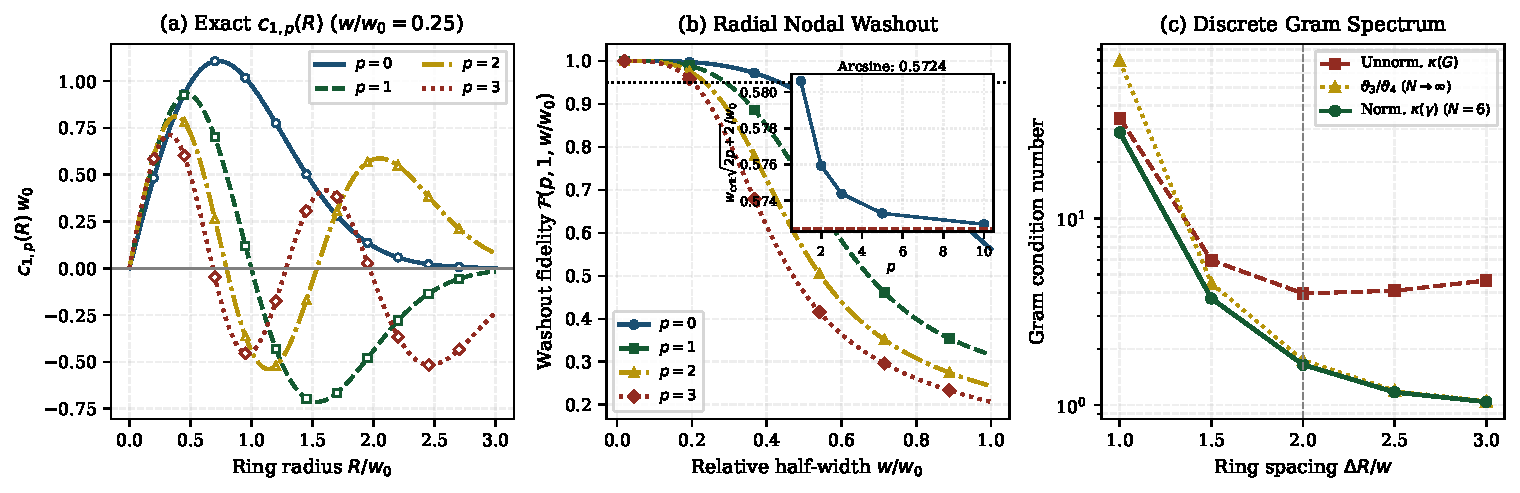
\includegraphics[width=0.99\textwidth]{fig4_lg_washout_gram.pdf}
  \caption{Laguerre--Gaussian expansion, nodal washout, and discrete Gram conditioning. (a) Closed-form $c_{1,p}(R)$ [Eq.~\eqref{eq:c_lp_exact}, curves] versus adaptive quadrature (markers, $p=0\text{--}3$, $w/w_0=0.25$, max error $1.08\times 10^{-15}$). (b) Washout fidelity $\mathcal{F}(p,1,w/w_0)$ with inset showing exact $\mathcal{F}=0.95$ roots converging to the WKB arcsine limit $0.57244$. (c) Monotonic unit-normalized $\kappa(\gamma)$ bounded by $\vartheta_3/\vartheta_4$ versus unnormalized $\kappa(G)$.}
  \label{fig:lg_gram}
\end{figure}

\section{Conclusions}
\label{sec:conclusions}

We have established a complete continuous Hilbert frame theory for physical finite-width perfect optical vortex beams. Azimuthal OAM sectors decouple strictly orthogonally, while radial overlap induces the isotropic Gaussian convolution frame operator $S_w = G_w * \cdot$ with optimal Bessel bound $B = 1$ on $L^2(\mathbb{R}^2)$ and sharp Paley--Wiener lower bound $A = \exp(-w^2 k_{\max}^2/2)$ on bandlimited optical subspaces $\mathcal{H}_{k_{\max}}$. By deriving the exact closed-form complex-waist Fresnel evolution $\Phi_{l,R}^{(z)}$, we proved $[S_w,\mathcal{U}_z] = 0$, establishing strict propagation invariance of the frame operator and frame bounds alongside the exact $\sigma_m^{+1}$-scaled Gouy-phase analyzer transformation. Finally, we validated the Tikhonov-regularized canonical dual on noisy $\mathrm{LG}_{2,1}$ deconvolution ($258.6\times$ MSE reduction), proved the exact $(p+1)$-term closed-form expansion $c_{l,p}(R)$ for all $p \ge 0$, derived the universal WKB arcsine radial resolution limit ($0.57244$), and bounded discrete concentric radial Gram conditioning uniformly by the Jacobi-theta ratio $\vartheta_3/\vartheta_4$. Photonic protocols applying these frame primitives to ring-core waveguides, atmospheric turbulence filtering, radial-qudit tomography, and aperture-invariant entanglement will be presented in a separate study.

\appendix
\section{Derivation of the Exact $(p+1)$-Term $\mathrm{LG}_{p,l}$ Expansion}
\label{app:lg_derivation}

Substituting Eq.~\eqref{eq:pvb_def} and $\psi_{p,l}(r,\phi)$ into $c_{l,p}(R) = \braket{\Phi_{l,R}}{\psi_{p,l}}$ and performing the azimuthal integral gives
\begin{equation}
  c_{l,p}(R) = 2\pi C_0 N_{p,l} e^{-R^2/w^2}\left(\frac{\sqrt{2}}{w_0}\right)^{\abs{l}} \int_0^\infty r^{\abs{l}+1} e^{-a_0 r^2} I_{\abs{l}}(b_R r)\,L_p^{\abs{l}}\!\left(\frac{2r^2}{w_0^2}\right)\dd r,
  \label{eq:app_int}
\end{equation}
with $a_0 = 1/w^2 + 1/w_0^2 = (w_0^2+w^2)/(w^2 w_0^2)$ and $b_R = 2R/w^2$, so $b_R^2/(4a_0) = R^2 w_0^2/[w^2(w_0^2+w^2)] = \zeta_R$ and $-R^2/w^2 + \zeta_R = -R^2/(w_0^2+w^2)$. Expanding $L_p^{\abs{l}}(2r^2/w_0^2) = \sum_{m=0}^p [(-1)^m/m!]\allowbreak\binom{p+\abs{l}}{p-m}(2/w_0^2)^m r^{2m}$ separates Eq.~\eqref{eq:app_int} into $(p+1)$ radial integrals. Each term closes via Gradshteyn--Ryzhik formula 6.631.1~\cite{Gradshteyn2014} (continued via $J_\nu(i b_R r) = i^\nu I_\nu(b_R r)$) with $\nu = \abs{l}$ and $(\mu+\nu)/2 = \abs{l}+m+1$:
\begin{equation}
  \int_0^\infty r^{\abs{l}+2m+1} e^{-a_0 r^2} I_{\abs{l}}(b_R r)\,\dd r = \frac{b_R^{\abs{l}}\,\Gamma(\abs{l}+m+1)}{2^{\abs{l}+1} a_0^{\abs{l}+m+1}\Gamma(\abs{l}+1)}\,{}_1F_1(\abs{l}+m+1;\,\abs{l}+1;\,\zeta_R).
\end{equation}
Applying Kummer's first transformation ${}_1F_1(\abs{l}+m+1;\,\abs{l}+1;\,\zeta_R) = e^{\zeta_R}\,{}_1F_1(-m;\,\abs{l}+1;\,-\zeta_R) = e^{\zeta_R}[m!\,\Gamma(\abs{l}+1)/\Gamma(\abs{l}+m+1)]L_m^{\abs{l}}(-\zeta_R)$ cancels $\Gamma(\abs{l}+m+1)/\Gamma(\abs{l}+1)$ and $m!$ identically. Collecting $(2/w_0^2)^m a_0^{-m} = [2w^2/(w_0^2+w^2)]^m = \xi^m$ and simplifying the remaining prefactor yields Eqs.~\eqref{eq:c_lp_exact}--\eqref{eq:A_pref}.

\begin{backmatter}
\bmsection{Funding}
This research received no external funding.

\bmsection{Acknowledgment}
The author acknowledges the use of standard symbolic and computational software tools for numerical verification and manuscript editing; all physical formulations, proofs, and interpretations are solely the responsibility of the author.

\bmsection{Disclosures}
The author declares no conflicts of interest.

\bmsection{Data availability}
Verification scripts, 50-digit quadrature tables, and figure-generation code underlying the results presented in this paper are openly available in Ref.~\cite{AyalaCodeV15}.
\end{backmatter}

\bibliography{references}

\end{document}
